\section{Contribution}

\subsection{Visualization framework}

\subsubsection{Structure}

One of the main issues that we had to be deal with at the beginning of the development process was the issue of how to integrate the visualizations into ProB 2.0. A functioning jetty server was already available, so we had to integrate our JavaScript visualizations into the existing framework. We ran into problems at the beginning, because a Java servlet is a singleton object. We needed to create a way to let the servlet know for which visualization it should be calculating. In order to do this, we created a session based servlet. When the user wants to open a visualization, the servlet is contacted. The servlet then creates a servlet responsible for the visualization and a unique session id. When a visualization sends a \texttt{GET} request, it includes its session id. The session based servlet then forwards the request to the the servlet that is responsible for the data calculations.

The visualization communicates with the servlet by setting up a polling interval. It tells the state space if it needs the complete data set or just the changes since the last polling interval. The servlet then responds by sending the correct data (see Figure \ref{communication}).

\begin{center}
\begin{figure}[h!]
\centering
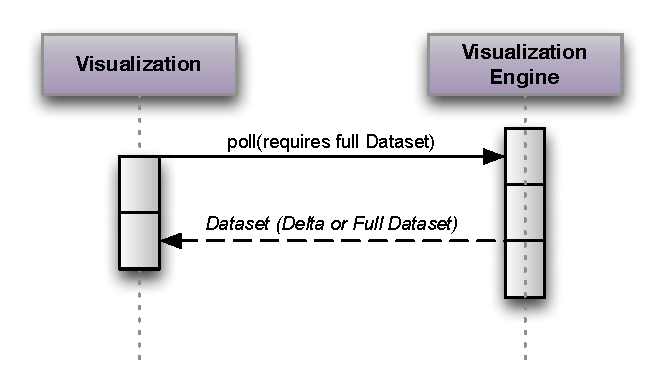
\includegraphics[width=14cm]{bilder/communication.pdf}
\caption{How visualizations communicate with the servlet that is responsible.}
\label{communication}
\end{figure}
\end{center}

The servlet is also connected to ProB 2.0 through the listener framework. Depending on the data that is needed for a particular visualization, the servlet registers either to receive notifications about changes in the current animation or about changes in the state space (see Figure \ref{programFlow}). Every time the servlet receives a new notification, the data needed for the visualization is recalculated.

\begin{center}
\begin{figure}[h!]
\centering
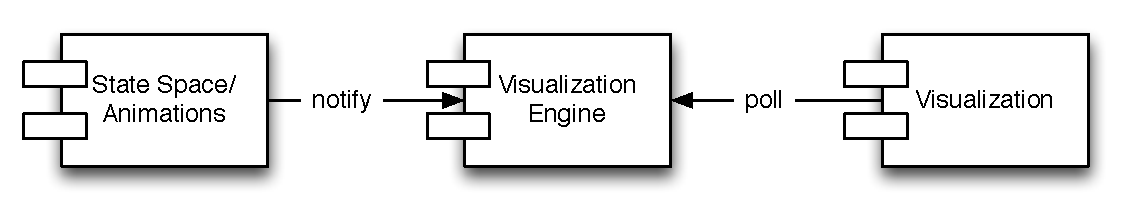
\includegraphics[width=14cm]{bilder/programFlow.pdf}
\caption{Model of the program flow.}
\label{programFlow}
\end{figure}
\end{center}

\subsubsection{User interaction with the visualizations}

Once we implemented a way to integrate the visualization servlets into the ProB 2.0 application, it was still necessary to implement an easy way for the user to interact with the visualizations. We wanted the user to be able to directly manipulate how the visualization appears. One of the main advantages of the D3 visualization framework is the flexibility that it provides for the developer. Using D3 selectors, it is possible for a developer to select and change the attributes of any of the elements of the visualization. We wanted the user to also be able to select and manipulate the visualization from within ProB. 

In order to allow the user to directly manipulate the DOM of the visualization, we decided to lift the functionality of the D3 selectors from the JavaScript level into the Java application. For this purpose, we defined a \texttt{Transformer} object. A \texttt{Transformer} consists mainly of a selector string and the \texttt{set} method. The \texttt{Transformer} is created by defining a selector based on the W3C Selectors API and calling the \texttt{set} method for every attribute that the user wants to manipulate. Because the \texttt{set} method returns the instance of the \texttt{Transformer}, it is possible chain the method calls together (see Lisiting \ref{javaTransformer}).

\lstset{language=java}
\begin{lstlisting}[caption=Define a \texttt{Transformer} in Java,label=javaTransformer]
// Select elements with ids "sroot" and "s1" and set their fill and stroke attributes
Transformer t = new Transformer("#sroot,#s1").set("fill","red").set("stroke","gray");
\end{lstlisting}

Every visualization servlet contains a list of \texttt{Transformers} that is sent to the visualization every time that it is polled. The visualization can then apply the \texttt{Transformers} to the DOM. We now needed a way for the user to create \texttt{Transformers} and add them to the visualization. It is possible to add a \texttt{Transformer} to a visualization servlet by calling the \texttt{apply} method present in all of the visualization servlets. When we create a new visualization servlet, we automatically create a variable in the Groovy console. The user can also use the \texttt{transform} closure available in the Groovy console to create \texttt{Transformers} which can then be applied to the visualization (see Listing \ref{transformer}).

\lstset{language=java}
\begin{lstlisting}[caption=Define rules for the transformation of visualization elements,label=transformer]
// Select elements with ids "sroot" and "s1" and set their fill and stroke attributes
x = transform("#sroot,#s1") {
        set "fill", "red"
        set "stroke", "gray"
}

// Apply to visualization
viz0.apply(x)
\end{lstlisting}

It is also possible to harness the power of the Groovy closure in order to create a Transformer that can be parameterized (see Listing \ref{transWclosure}).

\begin{lstlisting}[caption=Use Groovy closures to generate Transformers,label=transWclosure]
// Create a closure that can be parameterized
colorize = { selection, color ->
                transform(selection) {
                    set "fill", color
                }    
           }

// Color elements "sroot" and "s1" green
viz0.apply(colorize("#sroot,#s1", "green"))
\end{lstlisting}

The downside to this mechanism is that the user needs to have a good idea about the internal representation of the DOM in order to manipulate the visualizations. This mechanism is especially interesting for the state space visualization, so we spent more time defining the ids for the DOM elements. The SVG objects that are created using D3 are generated using the state ids and transition ids that are assigned by ProB. These element ids can be seen in Table \ref{tab:elements}.

\begin{table}[h!]
\caption{Generated Element Ids for Elements in State Space Visualization}
\label{tab:elements}
\begin{center}
\begin{tabular}{ | l | l | }
\hline
\textbf{Element} & \textbf{Generated Element Id} \\ \hline \hline
transition & \texttt{t + }\emph{transition id} \\ \hline
text on transition & \texttt{tt + }\emph{transition id} \\ \hline
state & \texttt{s + }\emph{state id} \\ \hline
text on state & \texttt{st + }\emph{state id} \\ \hline
\end{tabular}
\end{center}
\end{table}

It is also possible in ProB to filter a state space based on a predicate. This means that it is possible to give ProB a predicate and receive a list of state ids for which the given predicate holds. Ideally, however, we would want a \texttt{Transformer} based on a given predicate to be updated in the case that the state space changes.. For this purpose, we have introduced a \texttt{Transformer} that will be updated in the case that new states are added to the state space. The user can create such a transformer by specifying a predicate and a state space object (see Listing \ref{dynamicTransformer}). Currently, this will only update the state objects in the DOM, but in the future, the same concept can be applied for all of the different elements. 

\begin{lstlisting}[caption=Create a \texttt{Transformer} based on the states that match a given predicate,label=dynamicTransformer]
// Define your formula
predicate = "active\\/waiting={}" as ClassicalB

// Create a Transformer that will filter the given state space (saved in space0) according to the given predicate
x = transform(predicate, space_0 ) {
		set "fill", "blue"
		set "stroke", "white"
}

// Apply the Transformer to the visualization
viz0.apply(x)
\end{lstlisting}

\subsubsection{Extensibility}

In addition to creating visualizations that are useful to the user, we also wanted to make it easy for other developers to create similar visualizations. In order to help with this, we encapsuled certain elements common to all of the visualizations into a separate script. In order to have access to these elements, a developer simply needs to include the script before that of his visualization. Currently, there are two main elements included in this script. Firstly, the user can use the \texttt{createCanvas} function to create a D3 selection that includes support for zooming (see Listing \ref{canvas}). Secondly, if the user wants to be able to apply the \texttt{Transformers} that are described in the last section, there is a built in function to apply a list of \texttt{Transformers} to the visualization (see Listing \ref{applyStyling}). In the future, it will also be possible to add more functions to this script to make it even easier to create visualizations for ProB.

\begin{lstlisting}[caption=Append a D3 selection to an element that includes support for zooming,label=canvas]
var width = 600, height = 400;
var svg = createCanvas("#elementId", width, height);

// Append all further elements to this selection
svg.append(...);
\end{lstlisting}

\begin{lstlisting}[caption=Apply list of \texttt{Transformers} received from servlet,label=applyStyling]
// The servlet has been polled, and a response has been received
var styling = response.styling;

// ... Render the visualization
// ... Then apply the user defined styling
applyStyling(styling);
\end{lstlisting}


\subsection{Visualization of the State Space}

\subsubsection{Main visualization}

When a state space visualization is opened, the visualization servlet responsible for the state space visualization takes the state space associated with the current animation and extracts the information about the nodes and edges contained within the graph. This information is then processed by D3 using the force layout and rendered to create a visualization (see Figure \ref{zoomedOut}). As a basis for the visualization, we used the Force Directed Graph example created by Michael Bostock (see Appendix \ref{appendix:force}). 

\begin{center}
\begin{figure}[h!]
\centering
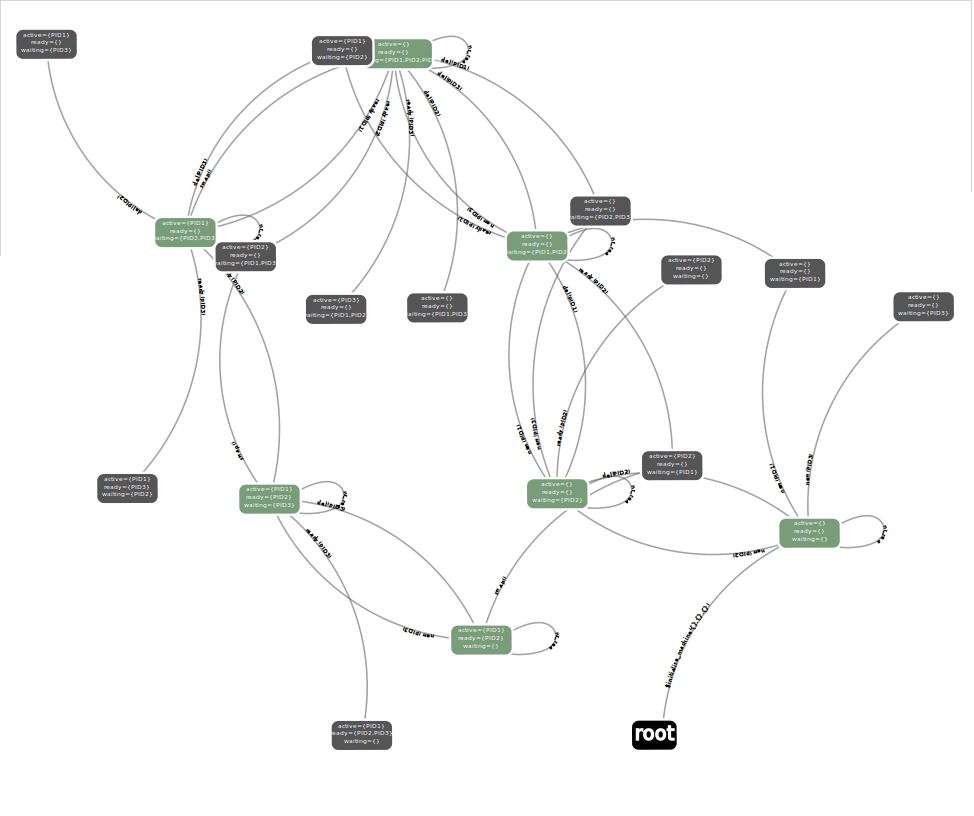
\includegraphics[width=13cm]{bilder/ss.png}
\caption{Visualization of a partially explored state space for the Scheduler example}
\label{zoomedOut}
\end{figure}
\end{center}

Unfortunately, the state space contains an extremely large amount of information that has to be processed. This includes the values of the variables and the invariant for every state in the graph and the names and parameters of the operations that correspond to every edge in the graph. Because of this, it is rather difficult to create a useful visualization of the whole state space because the user not only wants to inspect how the state space appears as a whole but also the individual states within the operation. As a proposed solution of this problem, we used the zoom functionality that is available in D3. The main problem was that if the visualization of the nodes was large enough for the user to read the values of the variable at the given state, it would no longer be possible to see the state space as a whole. Instead of trying to meet both requirements at once, we simply made the text that is printed on the node and edge objects very small. When the visualization is created, the user can inspect the graph as a whole how the graph appears as a whole. The text for the given nodes, however, is virtually indiscernable. If the user wants to inspect a particular node, they can do so by zooming into the visualization. The text is then larger, and the user can see the values of the variables for the given state and the out going transitions (see Figure \ref{onestate}). Then user can also click on the background of the visualization in order to pan through the visualization and inspect other nodes and edges. The visualization is also interactive. The user can grab a node and move it around to a desired position.

\begin{center}
\begin{figure}[h!]
\centering
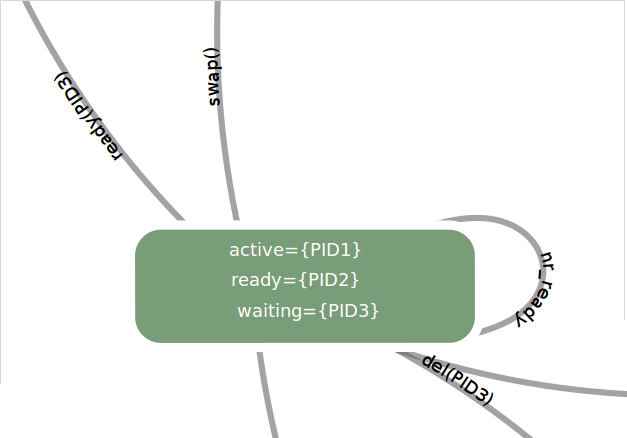
\includegraphics[width=14cm]{bilder/onestate.png}
\caption{By zooming in, the user can inspect individual nodes.}
\label{onestate}
\end{figure}
\end{center}

We had some performance issues that were associated with very large state spaces. The force layout keeps adjusting the graph until it reaches a fix point. The problem was that as the state space grew, there were more and more objects that had to be accounted for. The force layout just kept calculating and moving the the nodes. This didn't only affect the appearance of the visualization. It cost enough resources that the whole eclipse plugin would become unresponsive. A quick fix to this problem was adding a play/pause button to the upper left hand corner of the visualization (see Figure \ref{userSelect}). When the user is satisfied with the visualization and how it is laid out, he can press the pause button, and the graph will stop being rendered. When he presses the play button, the rendering will begin again. The iterative force layout keeps running in the background, so when the rendering begins again, the visualization has had time to stabilize.

When new states are added to the state space, these states are added to the graph when the visualization receives them in the next poll. The graph is then updated. This results in a nice animation.

Status about the invariant is a available in the graph based on the color of the nodes. If an invariant violation is present, the node is colored red. If the invariant is ok, the node is colored green. Otherwise, if the invariant has not yet been calculated for the given node, the node is colored gray.

The state spaces often grow exponentially. This is known as the state space explosion problem. For this reason, a visualization of the entire state space can often be a great deal too much information for a user to process at any given time. For this reason, we have also made smaller graphs available that are derived from the original state space and can be more useful for the user to visualize. The user can choose from these visualizations in the dropdown menu in the upper left hand corner (see Figure \ref{userSelect}).

\begin{center}
\begin{figure}[h!]
\centering
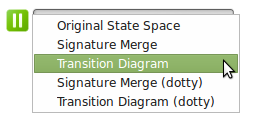
\includegraphics[width=8cm]{bilder/menu.png}
\caption{The user can select the desired visualization and play and pause the rendering.}
\label{userSelect}
\end{figure}
\end{center}

\subsubsection{Signature Merged State Spaces}

The signature merge algorithm is the first of two algorithms for reducing the state space that have been implemented in this work. The algorithm works by merging all of the states which have the same outgoing transitions. This creates a state space that is considerably smaller but that still preserves information about the operations that are enabled for a given state \cite{LeTu05_8} (see Figure \ref{sigmerge}). 

The graph that is generated with the signature merge algorithm differs based on the transitions that are of the interest of to the user. By default, all transitions are selected when the algorithm is run. However, it also possible to remove or readd transitions into the calculation of the algorithm. In order to allow the user to select the transitions of interest, we have implemented a small user interface that pops up when the user clicks on the settings icon (see Figure \ref{sigMergeUI}). The settings icon only becomes available when the user is in a mode dealing with the signature merge algorithm. The label for the nodes in this graph consists of a list of the outgoing transitions from the node and the number of states that have been merged into the node.  

\begin{center}
\begin{figure}[h!]
\centering
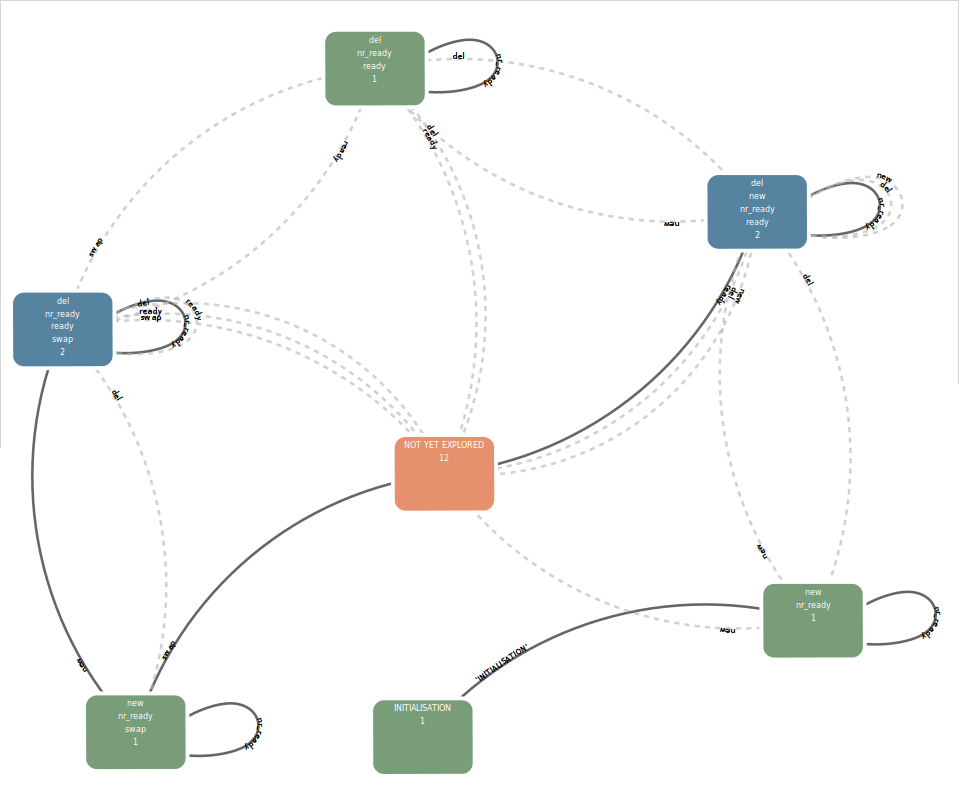
\includegraphics[width=14cm]{bilder/sigmerge.png}
\caption{D3 Visualization of signature merge for Scheduler example}
\label{sigmerge}
\end{figure}
\end{center}

\begin{center}
\begin{figure}[h!]
\centering
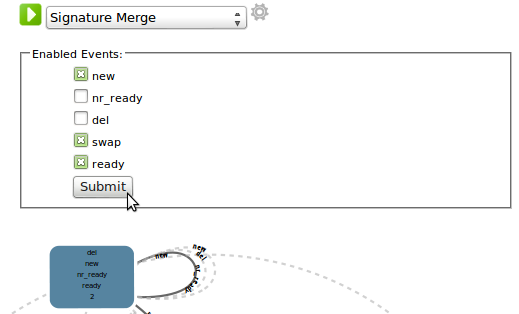
\includegraphics[width=8cm]{bilder/sigMergeUI.png}
\caption{User interface to chose events for signature merge.}
\label{sigMergeUI}
\end{figure}
\end{center}

If the user wants to use the GraphViz algorithms and rendering engine, there is also support for visualizing the DOT representation of the signature merged state space that is generated from ProB (see Figure \ref{sigmergeDotty}). This is done using the Viz.js JavaScript library. The same user interface is available for the GraphViz generated graph, and the visualization supports zooming and panning in the same way as the D3 powered visualizations do.

\begin{center}
\begin{figure}[h!]
\centering
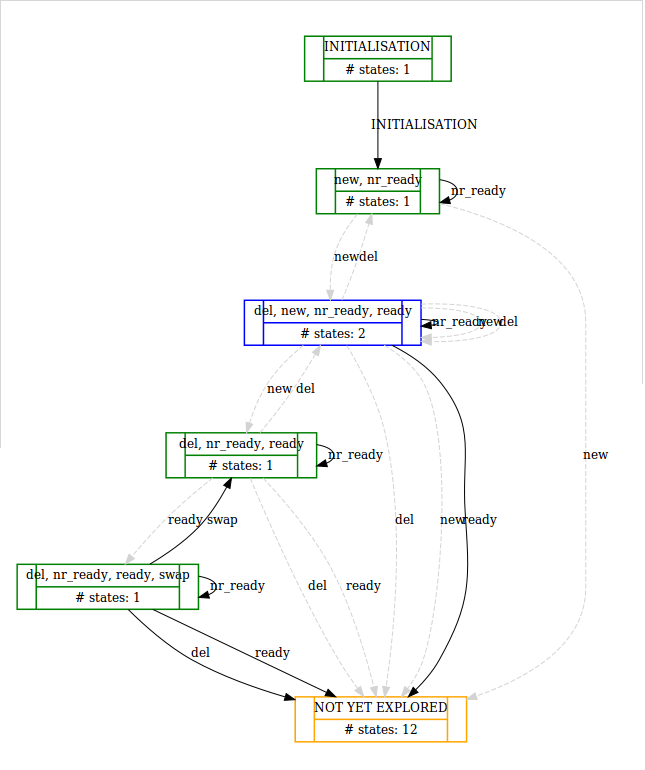
\includegraphics[width=14cm]{bilder/dotty-sigmerge.png}
\caption{GraphViz powered Visualization of the signature merge algorithm for the Scheduler example}
\label{sigmergeDotty}
\end{figure}
\end{center}

\subsubsection{Transition Diagrams}

The other reduction algorithm that is supported in this implementation is the creation of transition diagrams. In order to perform this algorithm, ProB receives an expression from the user. Then ProB calculates all of the possible solutions to the expression. These become the vertices in the graph. The edges in the graph show the transitions that change the value of the given expression to that of the value shown in the target state (see Figure \ref{transdiag}).

\begin{center}
\begin{figure}[h!]
\centering
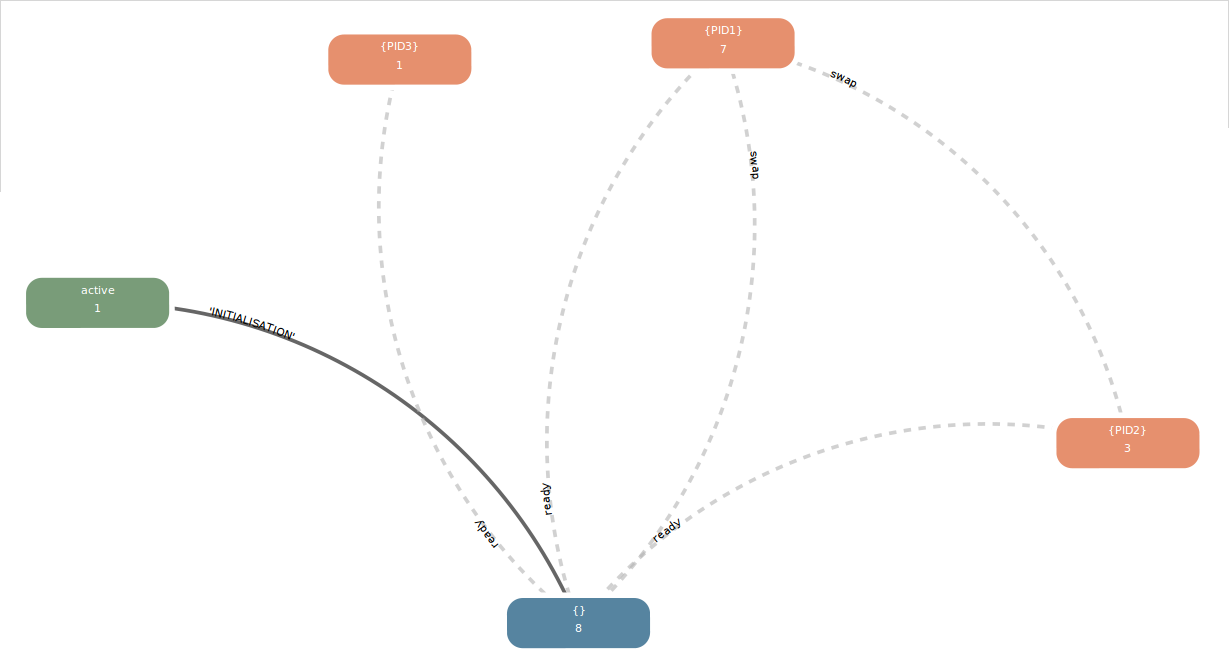
\includegraphics[width=14cm]{bilder/transdiag.png}
\caption{D3 Visualization of the transition diagram of \texttt{active} in Scheduler example}
\label{transdiag}
\end{figure}
\end{center} 

When the user chooses to create a transition diagram from the menu, a prompt appears. This is how the user can specify the initial expression for the calculation of the transition diagram. Once the graph is calculated and rendered, a text field appears next to the drop down menu (see Figure \ref{transDiagUI}). If the user wants to change the expression that is being visualized, they can input a new expression here and submit it. The algorithm will then be recalculated and the graph will be rerendered.

\begin{center}
\begin{figure}[h!]
\centering
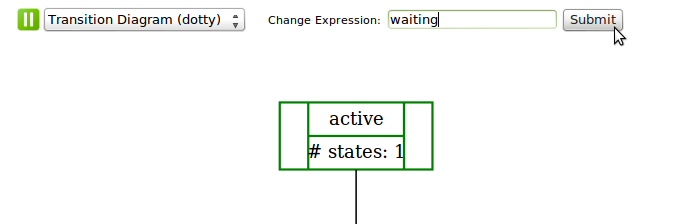
\includegraphics[width=8cm]{bilder/transDiag-UI.png}
\caption{The user can input a new expression to recalculate the transition diagram.}
\label{transDiagUI}
\end{figure}
\end{center}

If the user prefers the GraphViz represenation over the D3 powered visualization, it is also possible to generate a GraphViz based visualization for the transition diagram (see Figure \ref{transdiagDotty}). As with the signature merged state space, the UI for the GraphViz powered transition diagram is the same as that for the D3 powered visualization, and the visualization supports zooming and panning. Although the GraphViz algorithms are inherently offline, these visualizations make use of the visualization framework and are recalculated and rerendered every time that a change takes place within the state space.

\begin{center}
\begin{figure}[h!]
\centering
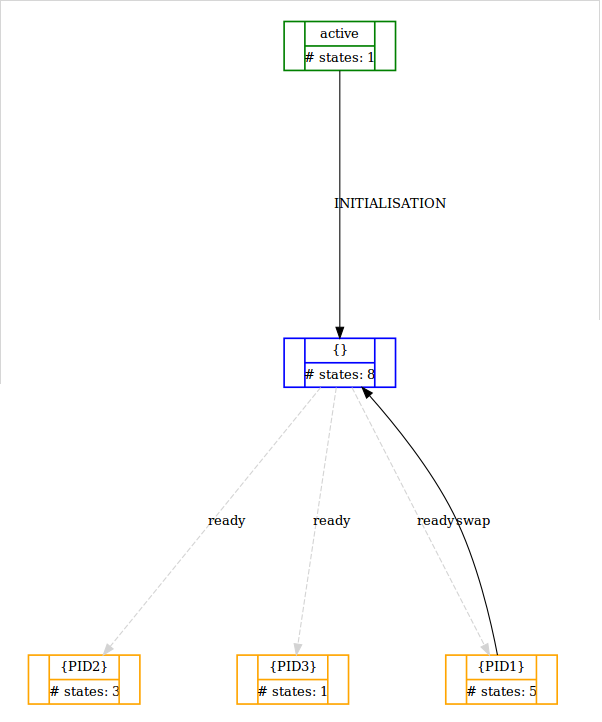
\includegraphics[width=14cm]{bilder/transdiag-dotty-wo.png}
\caption{GraphViz powered visualization of the transition diagram of \texttt{active} in Scheduler model}
\label{transdiagDotty}
\end{figure}
\end{center}

\subsection{Visualization of a B-type Formula}

ProB already supported the functionality of expanding a formula into its subformulas and finding its value at a given state. However, for any given formula, only the subformulas directly under the desired formula would be calculated. This algorithm was adapted so that all the subformulas are calculated automatically and a tree structure is built automatically. This structure is then cached, and can then be evaluated for any given state.

The final visualization is interactive (see Figure \ref{predicate}). If a formula has subformulas, the user can select it from within the visualization to expand or to retract the subformulas. The subformulas are always either predicates or expressions. If they are expressions, they are colored white or light grey depending on whether they have subformulas or not. If the formula is a predicate that has evaluated to true for the given formula, the node is colored green. If the formula is a predicated that has evaluated to false, node is colored in red. The value of the given formula is also printed beneath the formula. This allows the user to visually identify the parts of the formulas and their given values. 

\begin{center}
\begin{figure}[h!]
\centering
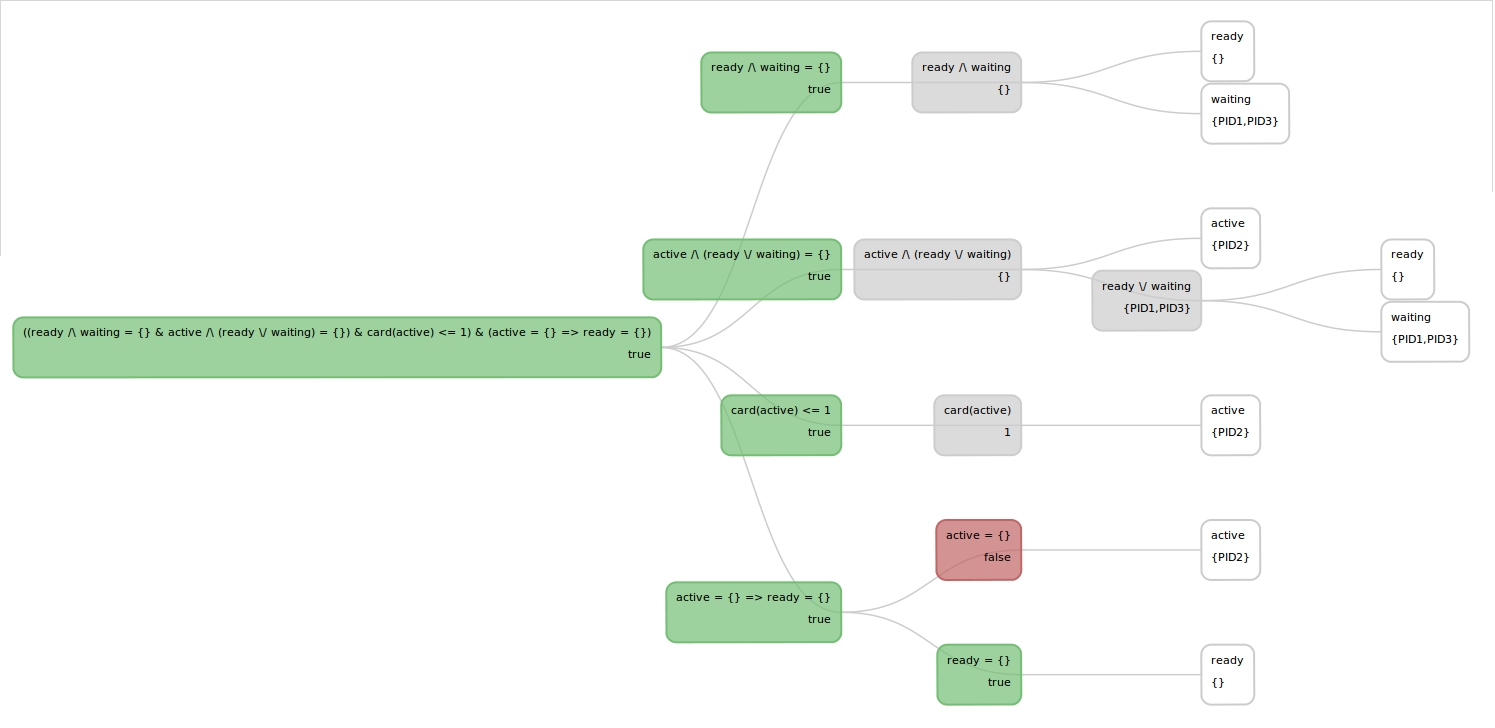
\includegraphics[width=14cm]{bilder/invariant.png}
\caption{Visualization of the invariant of the Scheduler model}
\label{predicate}
\end{figure}
\end{center}

In the implementation of the formula, the D3 tree layout is used. The expanding and collapsing of the nodes takes place with a simple JavaScript function. This visualization is based on the Collapsible Tree Layout from the D3 website (see Appendix \ref{appendix:tree}). By harnessing the power of the D3 zoom behavior, it is also possible to zoom in and out of the visualization and to pan the image to inspect it closer. The servlet responsible for the visualization implements a listener to identify if any changes in the animation occur. If they do, the formula is recalculated for the new current state, and the visualization is redrawn.

\subsection{Visualization of the Value of a Formula Over Time}

The last visualization that we have created in the course of this work is the visualization of the value of a given formula over the course of an animation.
Because a state is defined by the values that the variables take on when dealing with B type specification languages, it can be interesting to be able to examine the value of a variable over the course of a trace. This is particularly interesting when the concept of time is present in the model being animated. In this case, the user is often only interested in inspecting a particular variable to see how it changes over time. 

When the visualization is created, the user specifies the formula that is to be visualized. The user can also specify a second expression which will serve as the value for the time axis. Then it contacts ProB and extracts the value that the formlua takes on for each state in the list. This information is then processed by D3 to produce a simple line plot (see Figure \ref{timeVsValue}). Expressions that take on boolean values and integer values can be visualized. If the current state changes, the formula is recalculated and a new plot is produced.

\begin{center}
\begin{figure}[h!]
\centering
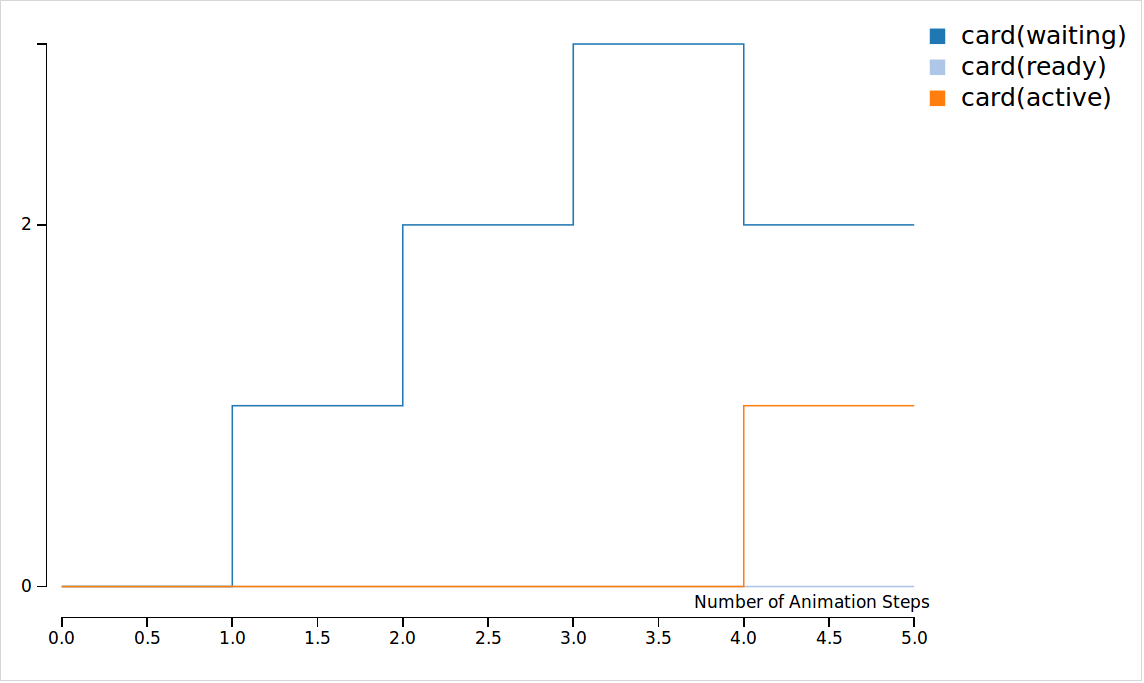
\includegraphics[width=14cm]{bilder/valueOverTime.png}
\caption{Visualization of value of the cardinality of the variables from the Scheduler model over the course of an animation.}
\label{timeVsValue}
\end{figure}
\end{center}

As seen in Figure \ref{timeVsValue}, it is possible to visualize multiple formulas at the same time. In order to add a formula to the visualization, the user can input a new formula in the text box in the upper left hand corner (see Figure \ref{timeVsValueUI}).

\begin{center}
\begin{figure}[h!]
\centering
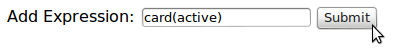
\includegraphics[width=8cm]{bilder/timeVValueUI.png}
\caption{The user can add an expression to the visualization.}
\label{timeVsValueUI}
\end{figure}
\end{center}